\chapter{\IfLanguageName{dutch}{Analyse van de cijfers}{Analysis of the figures}}%
\label{ch:analyse}

Allereerst heeft er een online vragenlijst plaatsgevonden. Daarna is de POC in gebruik genomen door diezelfde mensen als zij die de vragenlijst ingevuld hebben. Tenslotte is nogmaals een vragenlijst uitgestuurd om eventuele veranderingen of evoluties op te merken.

De éénentwintig bevraagde mensen zijn allen werkzaam in een sedentaire job. 42.9\% van de respondenten zijn tussen de 18 en 25 jaar oud, 42.9\% tussen de 25 en 35 jaar oud en de overige 14.3\% zijn tussen de 35 en 45 jaar oud. Deze bachelorproef kan dus geen conclusies trekken over mensen die zich buiten deze leeftijdsgroepen bevinden.

\section{Resultaten voor gebruik van Move-it!}

\subsection{Beweging}
Slechts 33.3\% van de bevraagde personen is tevreden met diens hoeveelheid dagelijkse beweging (zie figuur \ref{fig:dagelijkseBeweging}).

\begin{figure}[h]
    \caption[In welke mate vindt u van uzelf dat u dagelijks voldoende beweegt (op een schaal van 1 tot en met 5, gaande van 1 voor absoluut te weinig bewegen, tot en met 5 voor meer dan voldoende bewegen)?]{In welke mate vindt u van uzelf dat u dagelijks voldoende beweegt (op een schaal van 1 tot en met 5)?}
    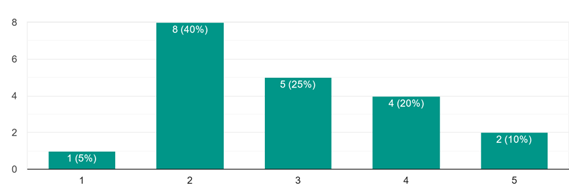
\includegraphics[width=1\textwidth]{DailyMovement}
    \label{fig:dagelijkseBeweging}
\end{figure}

Volgens de WHO moeten volwassenen tussen de 18 en 64 jaar oud wekelijks ongeveer 150 à 300 minuten met gemiddelde intensiteit sporten \autocite{Bull2020}.
Uit dit onderzoek is gebleken dat 47.5\% van de 18 à 45 jaar oude mensen dit voorgeschreven aantal niet halen. 19.1\% van hen sport meer dan 5 uur per week met gemiddelde intensiteit. Dit wil zeggen dat slechts 33.4\% van de mensen dit aangeraden aantal behaalt.

WHO stelt dat volwassenen van diezelfde leeftijdsgroep ongeveer 75 à 150 minuten met hoge intensiteit moeten sporten \autocite{Bull2020}.
52.4\% van de respondenten behaalt dit doel en 33.5\% van hen doet zelfs meer dan de aangeraden 150 minuten.

% TODO: naar conclusie verhuizen
In conclusie: vooral belang om te focussen op dagelijkse simpele beweging -> wordt minder behaald.

\subsection{Motivatie}

\begin{figure}[h]
    \caption[Zou u liever meer sporten dan u op dit moment doet?]{Zou u liever meer sporten dan u op dit moment doet?}
    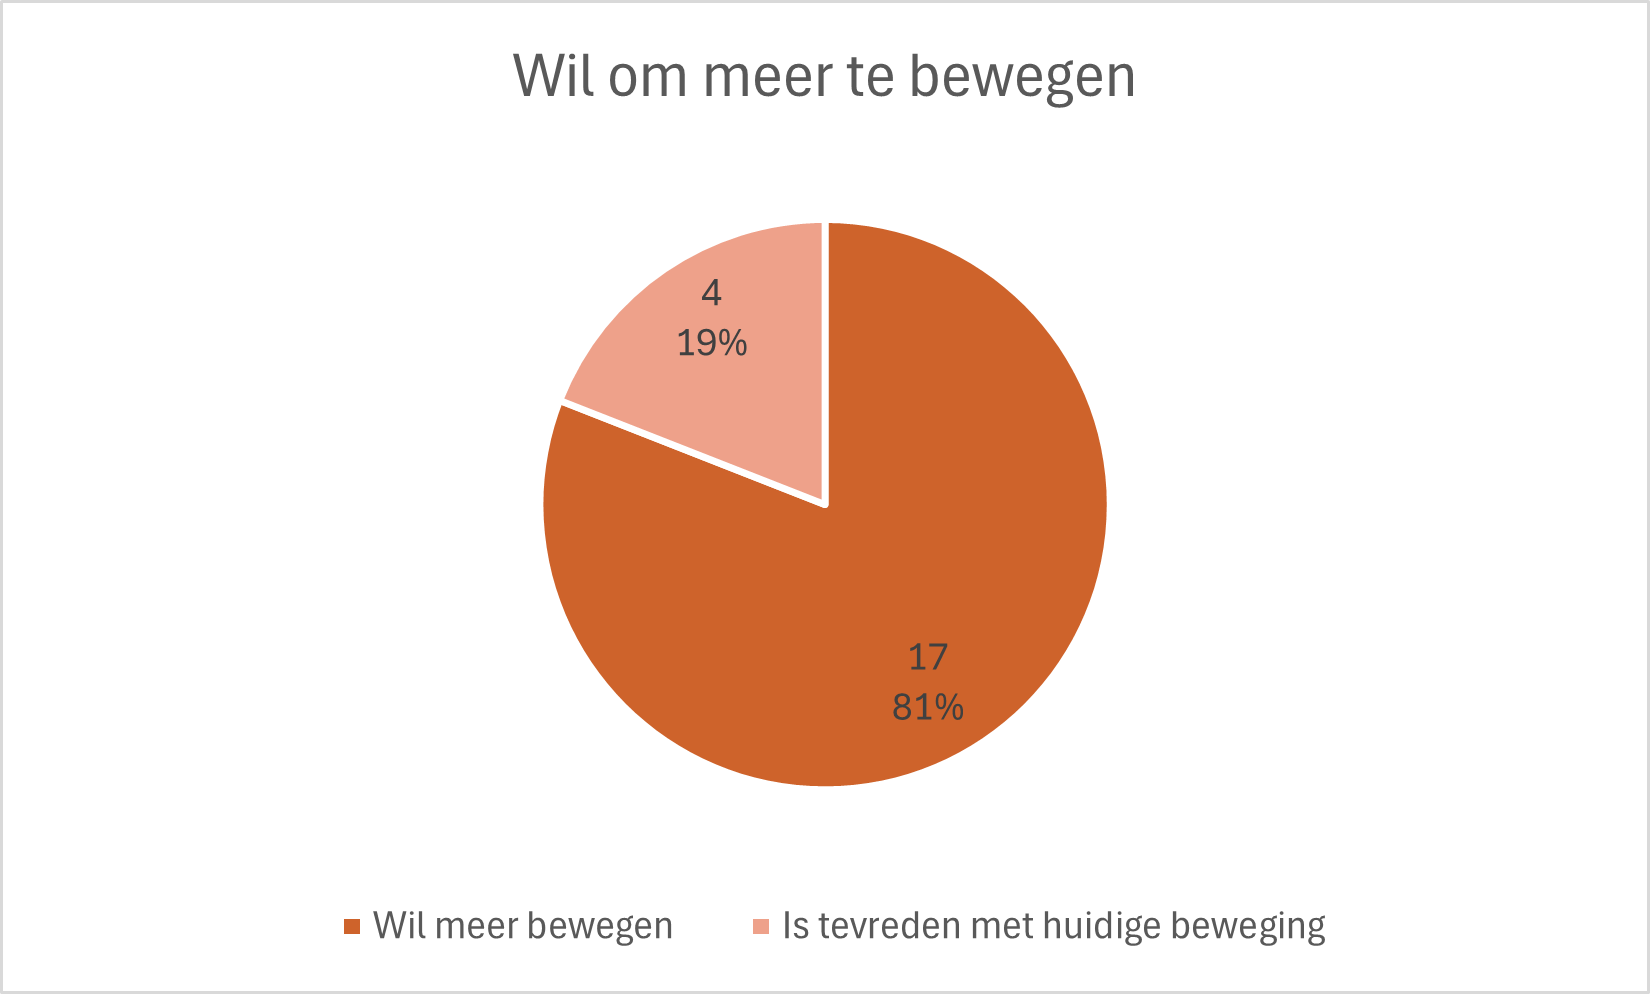
\includegraphics[width=1\textwidth]{MeerSporten}
    \label{fig:meerBewegen}
\end{figure}

Slechts vier van de éénentwintig mensen zijn tevreden met de hoeveelheid sport die ze op dit moment doen. Ruim 81\% is dus niet tevreden en zou liever meer sporten of bewegen (zie figuur \ref{fig:meerBewegen}).

Het grootste probleem voor mensen om meer te sporten, is tijd vinden. Daarnaast staan ook motivatie en wederkerende blessures in de weg. Een minderheid vindt ook geen plezier in het sporten (zie figuur \ref{fig:waarom}).

\begin{figure}[h]
    \caption[Wat houdt u op dit moment tegen om meer te sporten?]{Wat houdt u op dit moment tegen om meer te sporten?}
    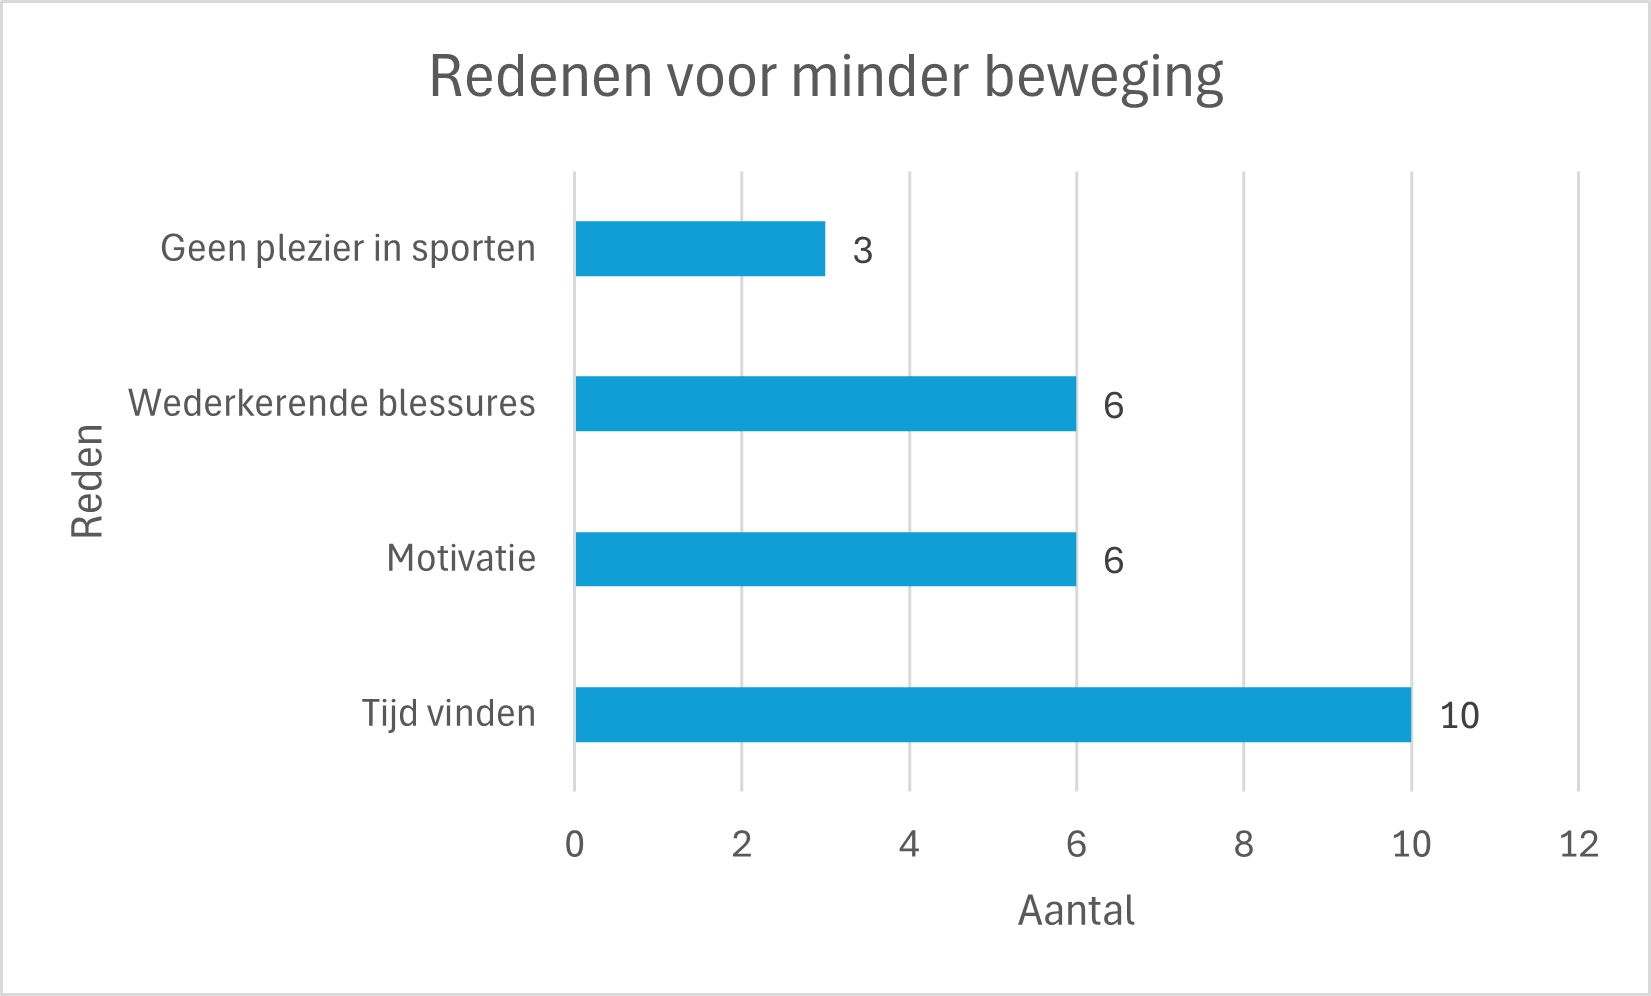
\includegraphics[width=1\textwidth]{Waarom}
    \label{fig:waarom}
\end{figure}

\subsection{Gamification}

Op vlak van het type gamification, is er een duidelijke voorkeur: 76.2\% van de respondenten verkiest een focus op persoonlijke vooruitgang.

Dit kan ook teruggevonden worden in wat belangrijk gevonden wordt in een sportapplicatie. 95.2\% vindt het meten van persoonlijke vooruitgang namelijk belangrijk en 71.4\% vindt ook technische gegevens zien over de activiteit een meerwaarde.

Het valt ook op dat sociale interacties, zoals likes, comments en volgers bijvoorbeeld, net als storend ervaren worden door 47.6\%, dit is tegenstrijdig met de literatuur.

Nog een tegenstrijdigheid die opvalt, is dat 38.1\% uitgedaagd en gemotiveerd wil worden door de applicatie, maar dat 42.9\% het storend vindt meldingen te ontvangen van een sportapplicatie. Dit wil dus zeggen dat deze motivatie op andere manieren dan gewoonlijk opgewekt moet worden.

\section{Sportresultaten}

Evolutie meten. Hoeveel percent haalt de voorgeschreven hoeveelheden.

Niet actieve gebruikers → sporten of gewoon niet ingeven?

\section{Resultaten na gebruik van Move-it!}

Nieuwe vragenlijst maken!

- focus op gevoel
- productiviteit?
- stress?
- competitief persoon? -> misschien enkel op competitieve mensen een invloed
- meer sporten in de toekomst?
- wat was anders dan andere sportapplicaties?
    - was dit beter of slechter?
- als u 1 ding zou kunnen veranderen, wat?